\documentclass[10pt]{article}
\usepackage{amsmath,amsthm,amssymb}
\usepackage{float}
\usepackage[norsk]{babel}
\usepackage[table]{xcolor}
\usepackage{color}
\usepackage{graphicx}
\usepackage{listings}
\usepackage{natbib}
\usepackage[utf8]{inputenc}
\usepackage{imakeidx}
\usepackage[a4paper]{geometry}
\usepackage[myheadings]{fullpage}
\usepackage{fancyhdr}
\usepackage{lastpage}
\usepackage{graphicx, wrapfig, subcaption, setspace, booktabs}
\usepackage[T1]{fontenc}
\usepackage[font=small, labelfont=bf]{caption}
\usepackage{fourier}
\usepackage[protrusion=true, expansion=true]{microtype}
\usepackage{url, lipsum}
\usepackage{tgbonum}
\usepackage{hyperref}
\usepackage{xcolor}
\usepackage[most]{tcolorbox}
\usepackage{mathtools}
\usepackage[page]{totalcount}
\usepackage{lastpage}

\newcommand{\HRule}[1]{\rule{\linewidth}{#1}}
\onehalfspacing
\setcounter{tocdepth}{5}
\setcounter{secnumdepth}{5}
\newcommand{\vect}[1]{\boldsymbol{#1}}

\definecolor{codegreen}{rgb}{0,0.6,0}
\definecolor{codegray}{rgb}{0.5,0.5,0.5}
\definecolor{codepurple}{rgb}{0.58,0,0.82}
\definecolor{backcolour}{rgb}{0.95,0.95,0.92}
\definecolor{skyblue}{rgb}{0.950, 1, 1}

\lstdefinestyle{mystyle}{
    backgroundcolor=\color{backcolour},   
    commentstyle=\color{codegreen},
    keywordstyle=\color{magenta},
    numberstyle=\tiny\color{codegray},
    stringstyle=\color{codepurple},
    basicstyle=\footnotesize,
    breakatwhitespace=false,         
    breaklines=true,                 
    captionpos=b,                    
    keepspaces=true,                 
    numbers=left,                    
    numbersep=5pt,                  
    showspaces=false,                
    showstringspaces=false,
    showtabs=false,                  
    tabsize=2,
    frame=single,
    %keywordstyle=\color{blue},
    language=Python,
    backgroundcolor = \color{skyblue}
}
 
\lstset{style=mystyle}
\lstset{
    basicstyle=\footnotesize\ttfamily,
  identifierstyle=\bfseries\color{green!40!black},
  commentstyle=\itshape\color{purple!40!black},
  keywordstyle=\color{blue},
  stringstyle=\color{orange},
}

\newcommand{\N}{\mathbb{N}}
\newcommand{\Z}{\mathbb{Z}}
 
\newenvironment{theorem}[2][Theorem]{\begin{trivlist}
\item[\hskip \labelsep {\bfseries #1}\hskip \labelsep {\bfseries #2.}]}{\end{trivlist}}
\newenvironment{lemma}[2][Lemma]{\begin{trivlist}
\item[\hskip \labelsep {\bfseries #1}\hskip \labelsep {\bfseries #2.}]}{\end{trivlist}}
\newenvironment{exercise}[2][Exercise]{\begin{trivlist}
\item[\hskip \labelsep {\bfseries #1}\hskip \labelsep {\bfseries #2.}]}{\end{trivlist}}
\newenvironment{problem}[2][Problem]{\begin{trivlist}
\item[\hskip \labelsep {\bfseries #1}\hskip \labelsep {\bfseries #2.}]}{\end{trivlist}}
\newenvironment{question}[2][Question]{\begin{trivlist}
\item[\hskip \labelsep {\bfseries #1}\hskip \labelsep {\bfseries #2.}]}{\end{trivlist}}
\newenvironment{corollary}[2][Corollary]{\begin{trivlist}
\item[\hskip \labelsep {\bfseries #1}\hskip \labelsep {\bfseries #2.}]}{\end{trivlist}}

\newenvironment{solution}{\begin{proof}[Solution]}{\end{proof}}
    
\makeindex[columns=3, title=Alphabetical Index, intoc]


% --------------------------------------------------------------
%                         Headers and footers
% --------------------------------------------------------------
\fancyhf{}
\pagestyle{fancy}
\rhead{Martin Soria Røvang}
\lhead{STA-2003-Tidsrekker}
\rfoot{Side \thepage \, av \pageref{LastPage}}
\renewcommand{\headrulewidth}{0.3pt}

\begin{document}
% --------------------------------------------------------------
%                         FRONTPAGE
% --------------------------------------------------------------
{\fontfamily{cmr}\selectfont
\title{ \normalsize \textsc{}
		\\ [3.0cm] % How much upper margin
		%\HRule{0.5pt} \\
        \LARGE \textbf{\uppercase{Obligatorisk Oppgave 1}
        \HRule{0.5pt} \\ [0.5cm]
        STA-2003-Tidsrekker
        %\HRule{2pt} \\ [0.5cm]
        \\
		\normalsize \today \vspace*{5\baselineskip}}
		}

        \date{}
\author{
		Martin Soria Røvang \\ 
        Universitetet i Tromsø \\}

% \begin{titlepage}
\clearpage\maketitle
\vspace{0.2\textheight}
{\centering
Inneholder \pageref{LastPage} \, sider, inkludert forside.\par
}
\thispagestyle{empty}
% \end{titlepage}

\newpage
\tableofcontents
% --------------------------------------------------------------
%                         Start here
% --------------------------------------------------------------

\newpage
\section{}
\subsection{a}


Hvit støy er en prosess som består av ukorrelerte tilfeldige variabler med forventing $\mu_{w} = 0$ og varians $\sigma^2_{w}$.
\begin{equation}
  W_{t} \thicksim WN(0,\sigma^2_{w})
\end{equation}

En hvit støy prosess man ofte kommer over er den Gaussiske hvite støy prosessen gitt ved,
\begin{equation}
  W_{t} \stackrel {iid}{\sim} N(0,\sigma^2_{w})
\end{equation}
som er identisk uavhengig fordelte punkter, denne prosessen er da strengt stasjonær.

\subsection{b}

Her har vi at $\hat{\rho}(h) \stackrel {d}{\sim}  \mathcal{N}(0,1/n)$, og dermed standardavvik $\sigma_{\hat{\rho}} = 1/\sqrt{n}$. Grensen der $95\%$ av verdiene er innenfor vil da være 1.96 standardavvik,
slik at $a = -1.96/\sqrt{n}$ og $b = 1.96/\sqrt{n}$.

\begin{equation}
  \mathcal{P}(-1.96/\sqrt{n} < \hat{\rho}(h) < 1.96/\sqrt{n}) = 95\%.
\end{equation}
Dette fordi,
\begin{equation*}
  P(Z > 1.96) = 0.025
\end{equation*}
der Z er standardnormalfordeling $Z = \frac{x - \mu}{\sigma}$, her er $\mu = 0$, siden ACF har fordelingen $\mathcal{N}(0,1/n)$
setter man inn får vi
\begin{equation*}
  P(\frac{x}{\sigma} > 1.96) = 0.025
\end{equation*}
løser for x gir,
\begin{equation*}
  P(x > 1.96\sigma) = 0.025
\end{equation*}
der sannsynligheten for x over 1.96$\sigma$ er 2.5\%.
Normalfordeling er symmetrisk rundt forventingen og vi vil derfor ha det samme for,
\begin{equation*}
  P(x < -1.96\sigma) = 0.025
\end{equation*}
Derfor vil verdier mellom dette intervallet gi $1 - (0.025 + 0.025)  = 0.95$

Ved bruk av python får vi samme resultat,
\begin{lstlisting}
from scipy.stats import norm
ss = norm.cdf(1.96) - norm.cdf(-1.96)
print(ss)
>> 0.95
\end{lstlisting}

I figur(\ref{ACF}) under kan man se verdiene på ACF over lag,

\begin{figure}[hbt!]
\center{
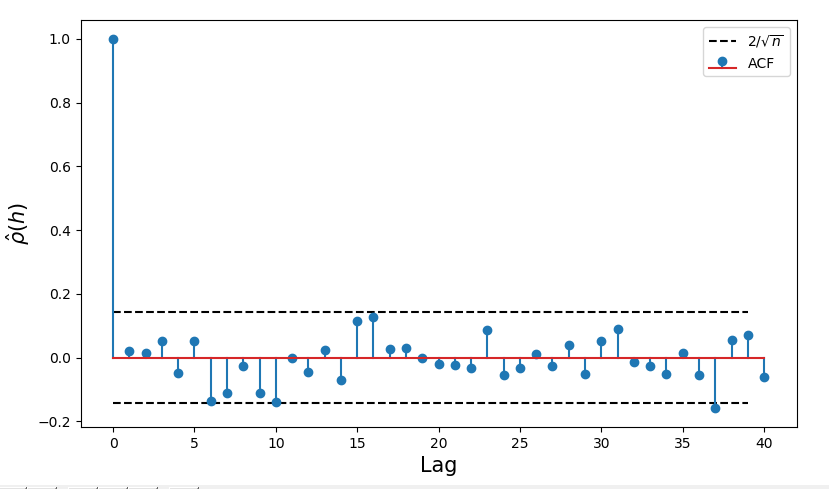
\includegraphics[scale=0.60]{ACF_plot.png}
}
\caption{ACF til en hvit støy prosess}
\label{ACF}
\end{figure}

Her kan man se at nesten alle verdiene ligger imellom $\pm$ 1.96 standardavvik.



\subsection{c}
Tidsrekke 1 er \emph{ikke konsistent} med hvit støy prosess fordi tidlige verdier er sterkt korrelert med de fremtidige.
\\
Tidsrekke 2 er \emph{konsistent} med hvit støy prosess fordi korrelasjonen med tidligere verdier er veldig svak og tilfeldig.
\\
Tidsrekke 3 er ikke hvit støy prosess fordi lag 1 er korrelert med tidligere verdier.

% \newpage

\section{}
\subsection{a}

En stokastisk prosess er Gaussisk hvis hvert endelig datapunkt for hver endelig tid er en tilfeldig variabel $X$ som følger en multidimensjonal gaussisk distribusjon. Derfor vil en multivariabel Gaussisk prosess ha stokastisk variabel $X \thicksim N(\vect{\mu},\vect{\Gamma})$,

\begin{equation}
  f_{\vect{X}}(x_{1},..,x_{N};t_{1},..,t_{N}) = \frac{1}{\sqrt{(2\pi)^{N} |\vect{\Gamma}|}}\exp\left[-\frac{1}{2}(\vect{x} - \vect{\bar{X}})^{T}\vect{\Gamma}^{-1}(\vect{x} - \vect{\bar{X}})  \right],
\end{equation}

hvor prosessen $\vect{x} = [x_{1},..,x_{N}]^{T}$, gjennomsnittsvektoren$\vect{\bar{X}} = [E[X_{1}],..,E[X_{N}]]^{T}$ og kovariansmatrisen er $\vect{\Gamma} = E[(\vect{x} - \vect{\bar{X}})(\vect{x} - \vect{\bar{X}})^{T}]$ der$|\cdot|$ angir determinanten.


\subsection{b}
Vet at $E[x_{t}] = 0$, hvis vi ser på varianser får vi,

\begin{equation*}
  Cov(x(t),x(s=t)) = \frac{\sigma^2}{2}(t^{2H} + t^{2H} - |t - t|^{2H}) = \sigma^2t^{2H}
\end{equation*}
Her ser vi at variansen er avhengig av tid og prosessen er dermed ikke stasjonær. Hvis variansen ikke hadde vært avhengig av tid måtte vi fortsatt se om autokovariansen kun var avhengig av \emph{lag} $|s - t| = h$, fordi variansen kun er et spesialtilfelle der $s = t$.



\subsection{c}

Har at $Cov(y_{t}, y_{s}) = E[y_{t}y_{s}] - E[y_{t}]E[y_{s}] $, der $E[y_{t}] = E[y_{s}] = 0$. Vi har da at,

\begin{equation*}
  Cov(X(t), X{s}) = E[X(t)X(s)]  = \frac{\sigma^2}{2}(t^{2H} + s^{2H} - |t-s|^{2H})
\end{equation*}
legger vi inn for $y(t)$ og $y(s)$ får vi $E[(x(t) - x(t-1))(x(s) - x(s-1))]$,
\begin{equation*}
  E[(x(t) - x(t-1))(x(s) - x(s-1))] = E[x(t)x(s) - E[x(t-1)x(s)] - E[x(s-1)x(t)] + E[x(t-1)x(s-1)]
\end{equation*}
løser opp og får,
\begin{align*}
  E[y_{t}y_{s}] = \frac{\sigma^2}{2}(t^{2H} + s^{2H} - |t-s|^{2H} - ((t-1)^{2H}\\ + s^2 - |(t-1)-s|^{2H})) - (t^{2H} + (s-1)^{2H} - |t-(s-1)|^{2H}))\\ + ((t-1)^{2H}(s-1)^{2H} - |(t-1)-(s-1)|^{2H})
\end{align*}
rydder vi opp får vi,

\begin{equation*}
  E[y_{t}y_{s}] = \frac{\sigma^2}{2}(-|t-s|^{2H} + |t-1-s|^{2H} - |t-s+1|^{2H} - |t-1-s+1|^{2H})
\end{equation*}
trekker sammen ledd,
\begin{equation*}
 Cov(y_{t}, y_{s}) = E[y_{t}y_{s}] = \frac{\sigma^2}{2}(|t-s+1|^{2H} + |t-1-s|^{2H} - 2|t-s|^{2H})
\end{equation*}
Variansen blir da,
\begin{equation*}
 Cov(y_{t}, y_{s=t}) = E[y_{t}y_{t}] = \frac{\sigma^2}{2}(|t-t+1|^{2H} + |t-1-t|^{2H} - 2|t-t|^{2H})
\end{equation*}
som blir,
\begin{equation*}
 \gamma(0) = \frac{\sigma^2}{2}(1 + 1 - 0) = \sigma^2
\end{equation*}
forenkler,
\begin{equation*}
 Cov(y_{t+h}, y_{t})= \gamma(h) = \frac{\sigma^2}{2}(|h+1|^{2H} + |h-1|^{2H} - 2|h|^{2H})
\end{equation*}

og tilslutt auto-korrelasjonsfunksjonen(ACF) $\rho(h) = \frac{\gamma(h)}{\gamma(0)}$,
\begin{equation*}
  \rho(h) = \frac{1}{2}(|h+1|^{2H} + |h-1|^{2H} - 2|h|^{2H})
\end{equation*}
som er det vi ville vise.


\subsection{d}

Vet at,
$H = 1/2$, $E[y_{t}] = 0$
da har vi,
\begin{equation}
  \gamma(h) = \frac{\sigma^2}{2}(|h+1| + |h-1| -2|h|)
\end{equation}
dette gir auto-kovariansfunksjonen gitt ved \emph{lag} h,
\[
 \gamma(h) = \begin{dcases}
      \sigma^2  & h = 0 \\
      0 & h \neq 0 \\
  \end{dcases}
\]
og auto-korrelasjonsfunksjonen(ACF) $\rho(h) = \frac{\gamma(h)}{\gamma(0)}$,
\[
 \rho(h) = \begin{dcases}
      1 & h = 0 \\
      0 & h \neq 0 \\
  \end{dcases}
\]
Denne følger en hvit støy prosess.


\subsection{e}
Denne prosessen er strengt stasjonær da vi vet at dette er en gaussisk prosess(iid).
Hvis den ikke hadde vært iid (identically independent distributed) hadde den vært svakt stasjonær fordi prosessen er avhengig av \emph{lag} h.



\subsection{f}
Løser opp for den asymptotisk like funkjonen,
\begin{equation*}
  \frac{1}{2}\frac{d^2}{d\tau^2}\tau^{2H}
\end{equation*}
som blir,
\begin{equation*}
  H(2H-1)\tau^{2(H-1)}
\end{equation*}
I figur(\ref{asymp}) under er ACF plottet med den asymptotiske funksjonen.
\begin{figure}[hbt!]
\center{
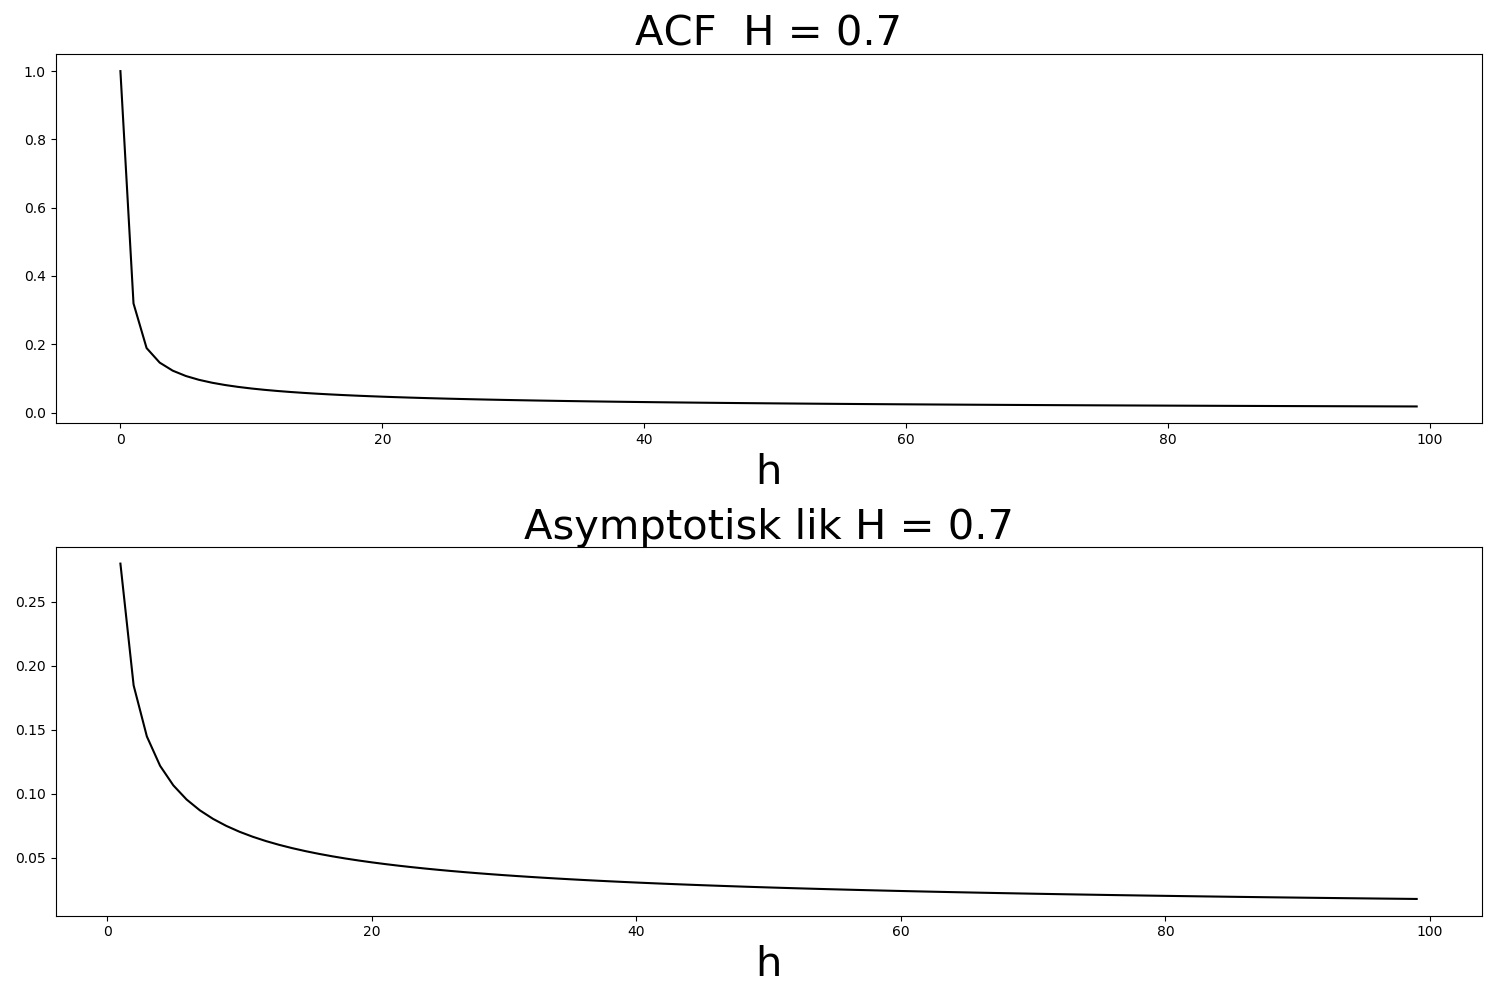
\includegraphics[scale=0.30]{Plots.jpg}
}
\caption{ACF og den som er asymptotisk like funksjonen}
\label{asymp}
\end{figure}

Her ser man at når $h -> \infty$ blir de mer lik. Her er $H = 0.7$ og her er det positiv men minkende korrelasjon.

I figur(\ref{asymp2}) er det samme plottet med verdi $H = 0.4$

\begin{figure}[hbt!]
\center{
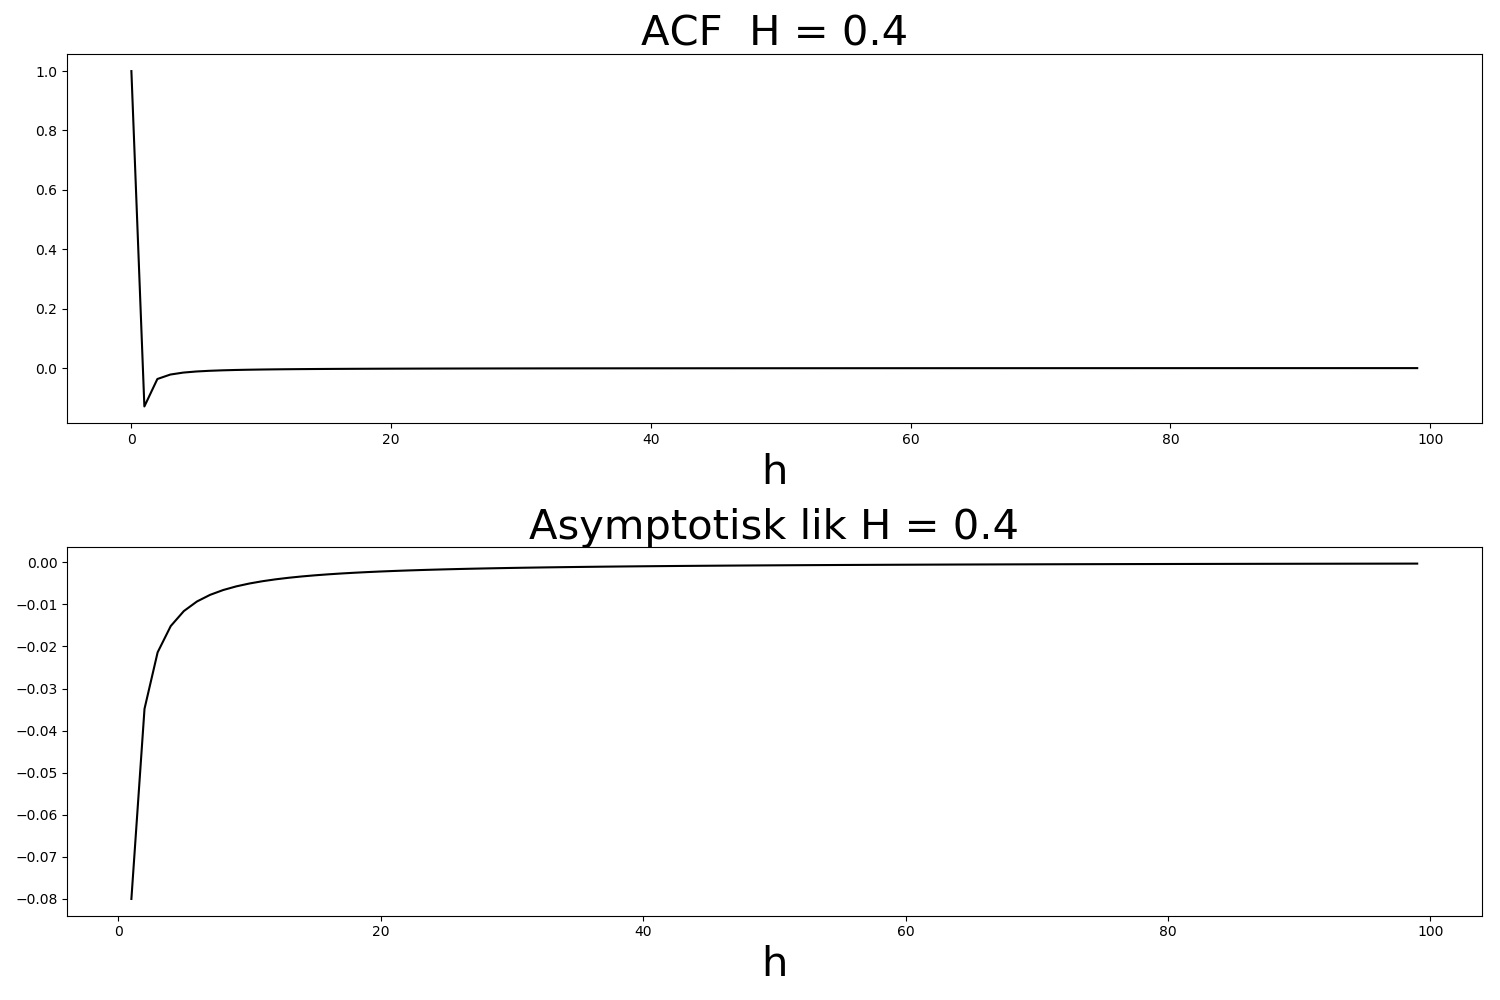
\includegraphics[scale=0.30]{Plots2.jpg}
}
\caption{ACF og den som er asymptotisk like funksjonen, $H = 0.4$}
\label{asymp2}
\end{figure}

Her ser man at når $h -> \infty$ blir de mer lik som tidligere, men med negativ korrelasjon i starten untatt $h = 0$.

Ved sammenligningstesten så divergerer summen $\sum_{h = 1}^{\infty} \rho(h)$, der $H > 1/2$ hvis vi bruker $\rho(h) \thicksim H(2H-1)\tau^{2(H-1)}$.

\subsection{g}
Har,
\begin{equation}
Cov(X(at),X(at)) = \frac{\sigma^2}{2}((at)^{2H} + (at)^{2H} - ( at - at)^{2H})
\end{equation}

løser opp og får,
\begin{equation}
  Cov(X(at),X(at)) = \sigma^2(at)^{2H}
  \end{equation}

for $a^{H}X(t)$ har vi,

\begin{equation}
  Cov(a^{H}X(t),a^{H}X(t)) = a^{2H}Cov(X(t), X(t)) = \sigma^2(at)^{2H}
  \end{equation}

Siden gaussisk prosess er kun definert ved første og andre ordens moment, og i dette tilfelle er første ordens moment $E[X(at)] = aE[X(t)] = E[a^{H}X(t)] = a^{H}E[X(t)] = 0$. Derfor har vi $[X(at)...X(at_{n})]\thicksim[a^{H}X(t)...a^{H}X(t_{n})]$.

%\newpage
\section{}
\subsection{a}

Starter med den lineære prosessen med støy som har 0 forventning og varians $\sigma_{w}^2$
\begin{equation}
  x_{t} = \beta_{0} + \beta_{1}t + w_{t}
\end{equation}


Forventing av $x_{t}$ blir,

\begin{equation*}
  E[x_{t}] = E[\beta_{0} + \beta_{1}t + w_{t}] = \beta_{0} + \beta_{1}t
\end{equation*}

fordi $\beta_{0} + \beta_{1}t$ leddene ikke er stokastiske og at forventning av det stokastiske leddet $w_{t}$ er null.

Siden forventning er avhengig av tid er prosessen ikke stasjonær.

\subsection{b}

Vi har differansen i første orden $\nabla ^1 x_{t}$ gitt ved,

\begin{equation*}
  \nabla x_{t} = x_{t} -  x_{t - 1} = (\beta_{0} + \beta_{1}t + w_{t}) - (\beta_{0} + \beta_{1}(t-1) + w_{t-1})
\end{equation*}

forkorter vi,

\begin{equation*}
  \nabla x_{t} = \beta_{1} + w_{t} - w_{t-1}
\end{equation*}


Forventning blir da,

\begin{equation*}
  E[\nabla x_{t}] = E[\beta_{1} + w_{t} - w_{t-1}] = \beta_{1}
\end{equation*}

Den er da ikke avhengig av tid, men vi må også se om autokovariansen er avhengig av tid, her kan vi se om prosessen er svakt stasjonær $\approx$ stasjonær (kun avhengig av tidsdifferansen/lag h).


\begin{equation*}
  \gamma_{x}(h) = E[(\nabla x_{t+h} - \mu)(\nabla x_{t} - \mu)]
\end{equation*}

her er $\mu = \beta_{1}$

\begin{equation}
  \gamma_{x}(h) = E[(\nabla x_{t+h} - \beta_{1})(\nabla x_{t} - \beta_{1})]
\end{equation}
Legger inn og får,
\begin{equation}
  \gamma_{x}(h) = E[(\beta_{1} + w_{t+h} - w_{t+h-1} - \beta_{1})(\beta_{1} + w_{t} - w_{t-1} - \beta_{1})]
\end{equation}

Forenkler,
 \begin{equation}
  \gamma_{\nabla x_{t}} = E[(w_{t+h} - w_{t+h-1})(w_{t} - w_{t-1})]
\end{equation}

dette blir,

  \begin{equation}
  \gamma_{\nabla x_{t}} = E[w_{t+h}w_{t} - w_{t+h-1}w_{t} - w_{t+h}w_{t-1} + w_{t+h-1}w_{t-1}]
\end{equation}

dette gir oss en stykkevis funksjon,

\[   
\gamma_{\nabla x_{t}} = 
   \begin{cases}
     2\sigma_{w}^2, &\quad h = 0\\
     -\sigma_{w}^2, &\quad |h| = 1 \\
     \text{0,} &\quad\text{eller.}
   \end{cases}
\]

Her er auto-kovariansfunksjonen kun avhengig av tidsdifferansen h, derfor er denne prosessen stasjonær.



\subsection{c}

Bytter vi ut støy leddet med en stasjonær prosess $y_{t}$ har vi forventningen,

\begin{equation*}
  E[\nabla x_{t}] = E[\beta_{1} + y_{t} - y_{t-1}] = \beta_{1}
\end{equation*}

fordi $E[y_{t}] = E[y_{t-1}] = \mu_{y}$.

Autokovariansen blir,

  \begin{equation*}
  \gamma_{\nabla x_{t}} = E[(x_{t+h} - x_{t+h - 1} - \mu)(x_{t} - x_{t- 1} - \mu)]
\end{equation*}

igjen er $\mu = \beta_{1}$. forenkler man dette får man,

  \begin{equation*}
  \gamma_{\nabla x_{t}} = E[(y_{t+h} - y_{t+h-1})(y_{t} - y_{t-1})]
\end{equation*}

som blir,

   \begin{equation*}
  \gamma_{\nabla x_{t}} = E[y_{t+h}y_{t} - y_{t+h-1}y_{t} - y_{t+h}y_{t-1} + y_{t+h-1}y_{t-1}]
\end{equation*}

forenkler,
\begin{equation*}
  \gamma_{\nabla x_{t}} = E[y_{t+h}y_{t}] - E[y_{t+h-1}y_{t}] - E[y_{t+h}y_{t-1}] + E[y_{t+h-1}y_{t-1}]
\end{equation*}

\begin{equation*}
  \gamma_{\nabla x_{t}} = \gamma(h) - \gamma(h - 1) - \gamma(h + 1) + \gamma(h)
\end{equation*}
som gir,
\begin{equation*}
  \gamma_{\nabla x_{t}} = 2\gamma(h) - \gamma(h - 1) - \gamma(h + 1)
\end{equation*}

Denne prosessen er derfor stasjonær fordi autokovariansen er avhengig av \emph{lag} h.







% --------------------------------------------------------------
%     Reference og appendix
% --------------------------------------------------------------
\newpage
\section{Appendix}
\section{Referanser}
\begingroup
\renewcommand{\section}[2]{}%
%\renewcommand{\chapter}[2]{}% for other classes
\bibliographystyle{plainnat}
\bibliography{bibl}
\endgroup


% --------------------------------------------------------------
%     You don't have to mess with anything below this line.
% --------------------------------------------------------------
 





\end{document}

